\section{Controller}

The controller is a Mealy machine used to sequence operations performed on the datapath.
Three main states exist to service the fetch, execute and interrupt stages.
Five sub states are used within the main states to further coordinate operation.
In practice this is implemented as a five bit word that containing $15$ operational states with $17$ dead states. 
The division was necessary for optimisation of the unit.


\begin{figure}[ht]
   \centering
    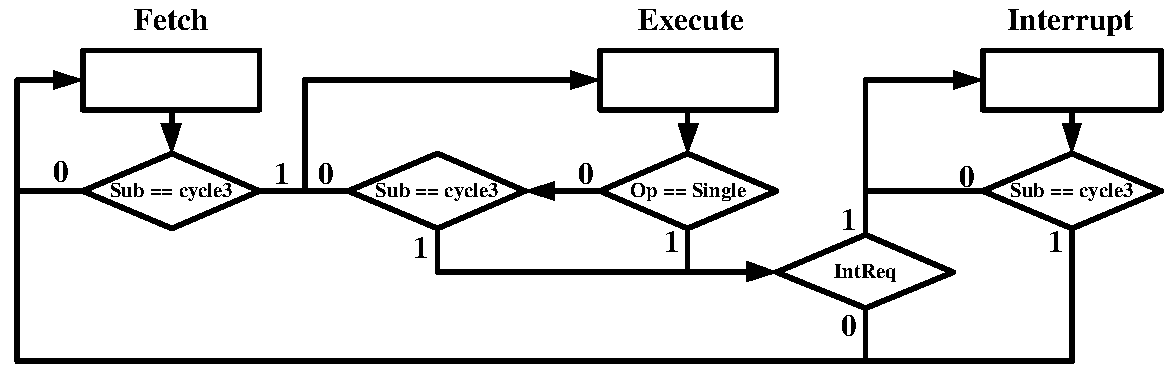
\includegraphics[width = 0.2\textwidth]{MainStateASM.pdf}
		\caption{ASM chart of contoller main states.}% \todo[inline]{Maybe change to IEEE symbols if we have time, AJR: we still have the eagle d-types but I think it would look a bit messy} }
   \label{fig:MainStateASM}
\end{figure}



Design of - simple statemachine?

Control signals - description, use of type defs?

Description of main states:

Fetch

Execute

Interrupt

Implementation of interrupts (flags, enable\dots)

Synthesis and layout - I/O config, magic vs Ledit maybe?
